\documentclass{scrreprt}
\usepackage{style}

\subject{5. Übung}
\title{389.055 Signale und Systeme 2 4.0}
\author{Byte Unit}
\uppertitleback{Unter GNU Free Document Lizenz}
\lowertitleback{\textcopyleft 2014 Byte Unit}
\date{\time}
%\publishers{}

\makeatletter
\AtBeginDocument{
    \hypersetup{
        pdftitle = {\@title},
        pdfsubject={\@subtitle},
        pdfauthor={\@author},
        pdfproducer={Latex (Debian/GNU Linux)},
        pdfkeywords={\@title, \@subject}
    }
}
\makeatother

\tikzstyle{point} = [draw, 
    fill=black,
    circle,
    inner sep=0pt]
\tikzstyle{block}=[rectangle,
    thick,
    minimum height=1cm,
    minimum width=1.5cm,
    draw=gray!80,
    fill=gray!20]    
\tikzstyle{sum} = [draw, 
    fill=gray!20,
    draw=gray!80,
    circle, 
    node distance=1cm]

\tikzstyle{input} = [coordinate]
\tikzstyle{output} = [coordinate]

\setcounter{tocdepth}{5}

\setcounter{chapter}{4}
\begin{document}
\chapter{Übung}
%\begin{uebsp}
\begin{Exercise}
    Berechnen Sie die Fouriertransformation $X(e^{j\theta})$ der folgenden Signale:
    \begin{enumerate}[a)]
        \item $\displaystyle x[n]=\alpha^n \sin\theta_0n\sigma[n]$ für $|\alpha|<1$
        \item $\displaystyle x[n]=2^n\sigma[-n]$
        \item $\displaystyle x[n]=\frac{\sin\frac{\pi}{2}n}{\pi
            n}\frac{\sin\frac{\pi}{4}n}{\pi n}$
        \item $\displaystyle x[n]=\left(\frac{1}{2}\right)^{|n|}$
        \item $\displaystyle x[n]=n\left(\frac{1}{2}\right)^{|n|}$
        \item $\displaystyle x[n]=(-1)^n$
        \item ~\\
            \begin{center}
                \begin{tikzpicture}
                    \begin{axis}[%
                        big,
                        axis y line=left,
                        legend style={at={(1,1.12), anchor=north west}},
                        xlabel={$n$},
                        ylabel={},
                        xmin=-15,   %i currently don't know why a xmin=-15
                                    %   results in xmin=20
                        xmax=15,
                        height=4cm,
                        domain={-20,20}]
                        \addplot+[ycomb,black,thick,mark=*,samples
                            at={-20,...,-10,10,11,...,20}] {0};
                        \addlegendentry[align=left]{$x[n]$};
                        \addplot+[ycomb,black,thick,mark=*,forget plot,samples
                            at={-10,...,0}] {(10+x)/10};
                        \addplot+[ycomb,black,thick,mark=*,forget plot,samples
                            at={1,...,10}] {(10-x)/10};
                    \end{axis}
                \end{tikzpicture}
            \end{center}
    \end{enumerate}
\end{Exercise}
\begin{Answer}
    \begin{enumerate}[a)]
        \item $\displaystyle x[n]=\alpha^n \sin\left(\theta_0n\right)\sigma[n]$ für
            $|\alpha|<1$:
            Mit der Eulerschen Formel kann man den $\sin$ in die Exponentialform
            bringen:
            \begin{definition}[Eulersche Formel]
                \[e^{j\varphi}=\cos(\varphi)+j\cdot\sin(\varphi)\]
                Bzw. 
                \[\sin x = \frac{e^{jx} - e^{-jx}}{2j}\;\;\;\text{ und
                    }\;\;\;\cos x = \frac{e^{jx} + e^{-jx}}{2}\]
            \end{definition}
            \[x[n]=\alpha^n\sin\left(\theta_0n\right)\sigma[n]
            =\underbrace{\alpha^n\sigma[n]}_{=b[n]}\frac{e^{j\theta_0n} - e^{-j\theta_0n}}{2j}
            =\left(\underbrace{e^{j\theta_0n}b[n]}_{=y[n]} -
                \underbrace{e^{-j\theta_0n}b[n]}_{=z[n]}\right)
            \frac{1}{2j}=\left(y[n]-z[n]\right)\frac{1}{2j}\]
            Zuerst berechne ich mir die Fouriertransformation von
            $b[n]=\alpha^n\sigma[n]$:
            \begin{uebsp_theory}
                Aus der Formelsammlung (Fouriertransformationspaare) folgt:
                \[a^n\sigma[n],\;\;|a|<1\;\;\multimapdotbothA\;\;\frac{1}{1-ae^{-j\theta}}\]
            \end{uebsp_theory}
            \[b[n]=\alpha^n\sigma[n]\multimapdotbothA
            B\left(e^{j\theta}\right)=\frac{1}{1-\alpha\cdot e^{-j\theta}}\]
            Anschließend kann man sich die Fouriertransformation von
            $y[n]=e^{j\theta_0n}b[n]$ berechnen:
            \begin{uebsp_theory}
                Aus der Formelsammlung (Fouriertransformation zeitdiskreter
                Signale) folgt:
                \[e^{j\theta_0n}x[n]\;\;\multimapdotbothA\;\;X\left(e^{j(\theta-\theta_0)}\right)\]
            \end{uebsp_theory}
            D.h. eine Multiplikation mit $e^{j\theta_0n}$ führt dazu, dass
            das $\theta$ durch $\theta-\theta_0$ ersetzt wird:
            \[y[n]=e^{j\theta_0n}b[n]\;\;\multimapdotbothA\;\;B\left(e^{j(\theta-\theta_0)}\right)=
                \;\;\fbox{ Subst.: $\theta-\theta_0=\tilde\theta$ }\;\;
                =B\left(e^{j(\tilde\theta)}\right)=\frac{1}{1-\alpha\cdot
                    e^{-j\tilde\theta}}\]
                    Rücksubstitution ($\tilde\theta=\theta-\theta_0$):
            \[B\left(e^{j(\tilde\theta)}\right)=B\left(e^{j(\theta-\theta_0)}\right)=\frac{1}{1-\alpha\cdot
            e^{-j(\theta-\theta_0)}}=Y\left(e^{j\theta}\right)\]
            Anschließend kann man sich die Fouriertransformation von
            $z[n]=e^{-j\theta_0n}b[n]$ berechnen (funktioniert analog zu $y[n]$):
            \[z[n]=e^{-j\theta_0n}b[n]\;\;\multimapdotbothA\;\;B\left(e^{j(\theta+\theta_0)}\right)=\frac{1}{1-\alpha\cdot
            e^{-j(\theta+\theta_0)}}=Z\left(e^{j\theta}\right)\]
            \begin{definition}[Linearitätseigenschaft der Fouriertransformation]
                \[a_1x_1[n]+a_2x_2[n]\multimapdotbothA
                a_1X_1(e^{j\theta})+a_2X_2(e^{j\theta})\]
            \end{definition}
            Aus der Linearitätseigenschaft folgt:
            \begin{eqnarray*}
                x[n]&=&\left(y[n]-z[n]\right)\frac{1}{2j}\;\;\multimapdotbothA\;\;
                \frac{1}{2j}\left(Y\left(e^{j\theta}\right)-Z\left(e^{j\theta}\right)\right)=
                X(e^{j\theta})\\
                X(e^{j\theta}) &=&
                \frac{1}{2j}\left(\frac{1}{1-\alpha\cdot e^{-j(\theta-\theta_0)}}
                    -\frac{1}{1-\alpha\cdot e^{-j(\theta+\theta_0)}}\right)\\
                X(e^{j\theta}) &=&
                    \frac{1}{2j}\left(\frac{1-\alpha\cdot
                    e^{-j(\theta+\theta_0)}-(1-\alpha\cdot
                e^{-j(\theta-\theta_0)})}{(1-\alpha\cdot e^{-j(\theta-\theta_0)})
                    (1-\alpha\cdot e^{-j(\theta+\theta_0)})}\right)\\
                X(e^{j\theta}) &=&
                    \frac{1}{2j}\left(\frac{\cancel 1-\alpha\cdot
                    e^{-j(\theta+\theta_0)}-\cancel 1+\alpha\cdot
                e^{-j(\theta-\theta_0)}}{1-\alpha\cdot e^{-j(\theta-\theta_0)}
            -\alpha\cdot e^{-j(\theta+\theta_0)}+\alpha^2\cdot
                e^{-j(\theta-\cancel{\theta_0}+\theta+\cancel{\theta_0})}}\right)\\
                X(e^{j\theta}) &=&
                \frac{1}{2j}\left(\frac{\alpha e^{-j\theta}\left(-
                    e^{-j(\theta_0)}+
            e^{j(\theta_0)}\right)}{1+\alpha^2\cdot
                e^{-j(2\theta)}-\alpha\cdot e^{-j\theta}\left( e^{j\theta_0}
        +e^{-j\theta_0}\right)}\right)\\
                X(e^{j\theta}) &=&
        \underbrace{\frac{\left(e^{j(\theta_0)}-e^{-j(\theta_0)}\right)}{2j}}_{=\sin\left(\theta_0\right)}\left(\frac{\alpha e^{-j\theta}}{1+\alpha^2\cdot
                e^{-j(2\theta)}-\frac{2}{2}\alpha\cdot e^{-j\theta}\left( e^{j\theta_0}
        +e^{-j\theta_0}\right)}\right)\\
                X(e^{j\theta}) &=&\frac{\alpha e^{-j\theta}\sin\left(\theta_0\right)}{1+\alpha^2\cdot
        e^{-j(2\theta)}-2\alpha\cdot e^{-j\theta}\underbrace{\frac{\left( e^{j\theta_0}
    +e^{-j\theta_0}\right)}{2}}_{=\cos\left(\theta_0\right)}}=
                \frac{\alpha e^{-j\theta}\sin\left(\theta_0\right)}{1+\alpha^2\cdot
        e^{-j(2\theta)}-2\alpha\cdot e^{-j\theta}\cos\left(\theta_0\right)}\\
            \end{eqnarray*}
        \item $\displaystyle x[n]=2^n\sigma[-n]$
            \begin{uebsp_theory}
                Aus der Formelsammlung (Fouriertransformationspaare) folgt:
                \[a^n\sigma[n],\;\;|a|<1\;\;\multimapdotbothA\;\;\frac{1}{1-ae^{-j\theta}}\]
            \end{uebsp_theory}
            \begin{eqnarray*}
                x[n]&=&2^n\sigma[-n]=\left(\frac{1}{2}\right)^{-n}\sigma[-n]
                    \;\;\fbox{Substituiere:$-n=\hat n$}\\
                x[-\hat n]&=&\left(\frac{1}{2}\right)^{\hat n}\sigma[\hat n]
            \end{eqnarray*}
            \begin{uebsp_theory}
                Aus der Formelsammlung (Fouriertransformation zeitdiskreter
                Signale) folgt:
                \[x[-n]\;\;\multimapdotbothA\;\;X\left(e^{-j\theta}\right)\]
            \end{uebsp_theory}
            Aus $\displaystyle x[-\hat n]\multimapdotbothA X\left(e^{-j\hat
                \theta}\right)$ und 
                $\displaystyle \left(\frac{1}{2}\right)^{\hat n}\sigma[\hat
                n]\multimapdotbothA \frac{1}{1-\frac{1}{2}e^{-j\hat\theta}}$ folgt:
            \begin{eqnarray*}
                x[-\hat n]&=&\left(\frac{1}{2}\right)^{\hat n}\sigma[\hat n] 
                    \;\;\Leftrightarrow\\
                    X\left(e^{-j\hat\theta}\right)&=&\frac{1}{1-\frac{1}{2}e^{-j\hat\theta}}
                    \;\;\fbox{Substituiere:$-\hat\theta=\theta$}\\
                    X\left(e^{j\theta}\right)&=&\frac{1}{1-\frac{1}{2}e^{j\theta}}
            \end{eqnarray*}

        \item $\displaystyle x[n]=\frac{\sin\frac{\pi}{2}n}{\pi
            n}\frac{\sin\frac{\pi}{4}n}{\pi n}$
            \[x[n]=\underbrace{\frac{\sin\frac{\pi}{2}n}{\pi
                n}}_{y[n]}\underbrace{\frac{\sin\frac{\pi}{4}n}{\pi n}}_{z[n]}\]
            \begin{uebsp_theory}
                Aus der Formelsammlung (Fouriertransformationspaare) folgt:
                \[\frac{\sin \alpha n}{\pi n}\multimapdotbothA
                X\left(e^{j\theta}\right)=\begin{cases}1&0\leq|\theta|\leq\alpha\\0&\alpha<|\theta|<\pi\end{cases}\]
            \end{uebsp_theory}
            Somit können wir uns $y[n]$ und $z[n]$ berechnen:
            \[y[n]=\frac{\sin \frac{\pi}{2} n}{\pi n}\multimapdotbothA
                Y\left(e^{j\theta}\right)=\begin{cases}1&0\leq|\theta|\leq\frac{\pi}{2}\\0&\frac{\pi}{2}<|\theta|<\pi\end{cases}\]
            \[z[n]=\frac{\sin \frac{\pi}{4} n}{\pi n}\multimapdotbothA
                Z\left(e^{j\theta}\right)=\begin{cases}1&0\leq|\theta|\leq\frac{\pi}{4}\\0&\frac{\pi}{4}<|\theta|<\pi\end{cases}\]
            \begin{definition}[Parsevalschen Beziehung (siehe 4.38 im Buch)]
                \[x_1[n]x_2[n]\;\;\multimapdotbothA\;\;\frac{1}{2\pi}\int_{-\pi}^{\pi}X_1\left(e^{j\eta}\right)X_2\left(e^{j(\theta-\eta)}\right)d\eta\]
            \end{definition}
            Mit der Parsevalschen Beziehung folgt:
            \[x[n]=y[n]z[n]\;\;\multimapdotbothA\;\;\frac{1}{2\pi}\int_{-\pi}^\pi
            Y\left(e^{j\eta}\right)\cdot
            Z\left(e^{j\left(j(\theta-\eta)\right)}\right)d\eta\]
            Da gilt: $Y\left(e^{j\eta}\right)=1$ für $|\eta|\leq\frac{\pi}{2}$
                sonst $0$. 
            Somit können wir das Integral etwas vereinfachen und die Grenzen
            etwas anpassen:
            \[X\left(e^{j(\theta-\eta)}\right)=\frac{1}{2\pi}\int_{-\frac{\pi}{2}}^{\frac{\pi}{2}} Z\left(e^{j(\theta-\eta)}\right)d\eta\]
            Substituiere: $\beta=\theta-\eta\;\;\Rightarrow\;\;d\beta=-d\eta$\\
            Grenzen substituieren: $\beta=\theta-\frac{\pi}{2}$ bzw.
            $\beta=\theta+\frac{\pi}{2}$.

            \[X\left(e^{j\theta}\right)=\frac{1}{2\pi}\int_{\theta+\frac{\pi}{2}}^{\theta-\frac{\pi}{2}}Z
            \left(e^{j\beta}\right)(-d\beta)=-\frac{1}{2\pi}\int_{\theta+\frac{\pi}{2}}^{\theta-\frac{\pi}{2}}Z
            \left(e^{j\beta}\right)d\beta\]
            wenn man die Grenzen vertauscht, enspricht das einer Multiplikation
            mit $(-1)$:
            \[X\left(e^{j\theta}\right)=\frac{1}{2\pi}\int_{\theta-\frac{\pi}{2}}^{\theta+\frac{\pi}{2}}Z
            \left(e^{j\beta}\right)d\beta\]

            Beim Lösen der Fallunterscheidung hilft eine Grafik:\\
            \raisebox{-.5\height}{
            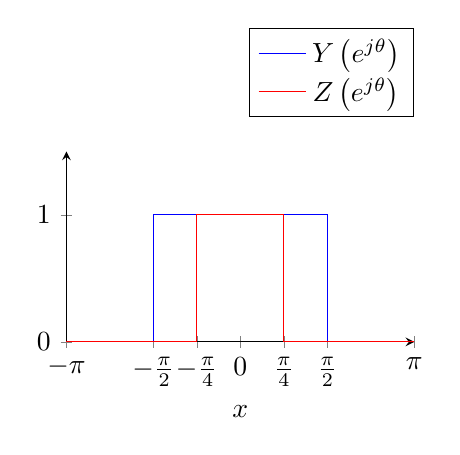
\begin{tikzpicture}
            \begin{axis}[
                domain=-pi:pi,
                axis x line=bottom, % no box around the plot, only x and y axis
                axis y line=left, % the * would suppress the arrow tips
                xlabel={$x$},
                ymax=1.5,
                legend style={at={(1,1.65), anchor=north west}},
                samples=50,
                height=4cm,
                width=6cm,
                xtick={-3.1416, -1.5708, -0.7854, 0, 0.7854, 1.5708, 3.1416},
                xticklabels={$-\pi$,$-\frac{\pi}{2}$,$-\frac{\pi}{4}$,$0$,$\frac{\pi}{4}$,$\frac{\pi}{2}$,$\pi$,$2\pi$},
                ytick={0,1},
                yticklabels={0,1},
                clip=false]
                \addplot[mark=none, color=blue] coordinates {
                    (-pi,0)
                    (-pi/2,0)
                    (-pi/2,1)
                    (pi/2,1)
                    (pi/2,0)
                    (pi,0)
                };
                \addlegendentry[align=left]{$Y\left(e^{j\theta}\right)$};
                \addplot[mark=none, color=red] coordinates {
                    (-pi,0)
                    (-pi/4,0)
                    (-pi/4,1)
                    (pi/4,1)
                    (pi/4,0)
                    (pi,0)
                };
                \addlegendentry[align=left]{$Z\left(e^{j\theta}\right)$};
            \end{axis}a
            \end{tikzpicture}}
            \raisebox{-.5\height}{$\xRightarrow{gefaltet}$}
            \raisebox{-.5\height}{
            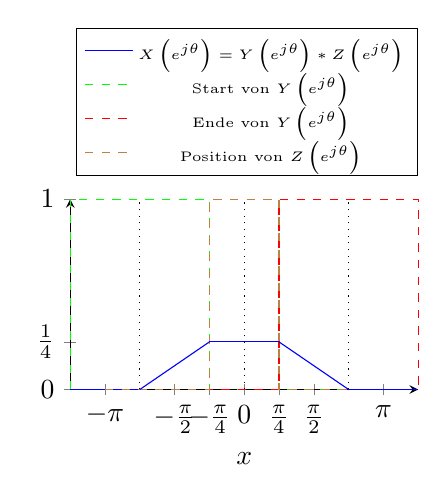
\begin{tikzpicture}
            \begin{axis}[
                    domain=-5*pi/4:5*pi/4,
                axis x line=bottom, % no box around the plot, only x and y axis
                axis y line=left, % the * would suppress the arrow tips
                xlabel={$x$},
                ymax=1,
                legend style={at={(1,1.9), anchor=north west,font=\tiny}},
                samples=50,
                height=4cm,
                width=6cm,
                xtick={-3.1416, -1.5708, -0.7854, 0, 0.7854, 1.5708, 3.1416},
                xticklabels={$-\pi$,$-\frac{\pi}{2}$,$-\frac{\pi}{4}$,$0$,$\frac{\pi}{4}$,$\frac{\pi}{2}$,$\pi$,$2\pi$},
                ytick={0,0.25,1},
                yticklabels={$0$,$\frac{1}{4}$,$1$},
                clip=false]
                \addplot[thin, smooth, blue,domain=-5*pi/4:-3*pi/4] {0};
                \addlegendentry[align=left]{$X\left(e^{j\theta}\right)=Y\left(e^{j\theta}\right)*Z\left(e^{j\theta}\right)$};
                \addplot[dashed,mark=none, color=green] coordinates {
                    (-5*pi/4,0)
                    (-5*pi/4,1)
                    (-pi/4,1)
                    (-pi/4,0)
                    (pi,0)
                };
                \addlegendentry[align=left]{Start von $Y\left(e^{j\theta}\right)$};
                \addplot[dashed,mark=none, color=red] coordinates {
                    (-pi,0)
                    (pi/4,0)
                    (pi/4,1)
                    (5*pi/4,1)
                    (5*pi/4,0)
                };
                \addlegendentry[align=left]{Ende von $Y\left(e^{j\theta}\right)$};
                \addplot[dashed,mark=none, color=brown] coordinates {
                    (-pi,0)
                    (-pi/4,0)
                    (-pi/4,1)
                    (pi/4,1)
                    (pi/4,0)
                    (pi,0)
                };
                \addlegendentry[align=left]{Position von $Z\left(e^{j\theta}\right)$};

                \addplot[thin, smooth, blue,domain=-3*pi/4:-pi/4] {3/8+x/(2*pi)};
                \addplot[thin, smooth, blue,domain=-pi/4:pi/4] {1/4};
                \addplot[thin, smooth, blue,domain=pi/4:3*pi/4] {3/8-x/(2*pi)};
                \addplot[thin, smooth, blue,domain=3*pi/4:5*pi/4] {0};

                \addplot[dotted, mark=none, color=black] coordinates {
                    (0,0)
                    (0,1)
                };
                \addplot[dotted, mark=none, color=black] coordinates {
                    (-3*pi/4,0)
                    (-3*pi/4,1)
                };
                \addplot[dotted, mark=none, color=black] coordinates {
                    (3*pi/4,0)
                    (3*pi/4,1)
                };

            \end{axis}
            \end{tikzpicture}}
            
            Wenn man sich vorstellt, dass $Y\left(e^{j\theta}\right)$ sich
            entlang der x-Achse nach rechts bewegt, dann sieht man in der
            Grafik, dass die Kurve $X\left(e^{j\theta}\right)$ ansteigt, wenn
            $Y\left(e^{j\theta}\right)$ die grüne Position eingenommen hat, dass
            sie stagniert, wenn der Mittelpunkt von $Y\left(e^{j\theta}\right)$
            den Wert $-\frac{\pi}{4}$ erreicht hat, dass sie wieder fällt,
            wenn der Mittelpunkt $\frac{\pi}{4}$ erreicht hat und dass sie $0$
            wird, wenn die rote Position angenommen wurde.

            Weiters ist ersichtlich, dass es somit 5 verschiedene
            Intervalle gibt:
            \begin{enumerate}
                \item $\displaystyle -\pi<\theta<-\frac{3\pi}{4}$
                \item $\displaystyle -\frac{3\pi}{4}<\theta<-\frac{\pi}{4}$
                \item $\displaystyle -\frac{\pi}{4}<\theta<\frac{\pi}{4}$
                \item $\displaystyle \frac{\pi}{4}<\theta<\frac{3\pi}{4}$
                \item $\displaystyle \frac{3\pi}{4}<\theta<\pi$
            \end{enumerate}
            Somit kann das Integral aufgespalten werden:\\
            \begin{minipage}{\linewidth}
            \[X\left(e^{j\theta}\right)=\frac{1}{2\pi}\int_{\theta-\frac{\pi}{2}}^{\theta+\frac{\pi}{2}}Z
                \left(e^{j\beta}\right)d\beta=
                \underbrace{\frac{1}{2\pi}\int_{\theta-\frac{\pi}{2}}^{-\frac{\pi}{4}}Z\left(e^{j\beta}\right)d\beta}
                    _{=0\text{, wenn }\theta\notin[\frac{\pi}{4},\frac{3\pi}{4}]
                        \;siehe \footnote{Da $Z\left(e^{j\theta}\right)$ nur für
                        $-\frac{\pi}{4}\leq\theta\leq\frac{\pi}{4}$ definiert ist,
                        folgt: $-\frac{\pi}{4}\leq\theta-\frac{\pi}{2}\leq\frac{\pi}{4}\;\;\Rightarrow\;\;
                            \frac{\pi}{4}\leq\theta\leq\frac{3\pi}{4}$}}+
                \underbrace{\frac{1}{2\pi}\int_{-\frac{\pi}{4}}^{\frac{\pi}{4}}Z\left(e^{j\beta}\right)d\beta}
                    _{=0\text{, wenn }\theta\notin[-\frac{\pi}{4},\frac{\pi}{4}]
                        \;siehe \footnote{Da $Z\left(e^{j\theta}\right)$ nur für
                        $-\frac{\pi}{4}\leq\theta\leq\frac{\pi}{4}$ definiert ist,
                        folgt: $-\frac{\pi}{4}\leq\theta\leq\frac{\pi}{4}$}}+
                \underbrace{\frac{1}{2\pi}\int_{\frac{\pi}{4}}^{\theta+\frac{\pi}{2}}Z\left(e^{j\beta}\right)d\beta}
                    _{=0\text{, wenn }\theta\notin[-\frac{3\pi}{4},-\frac{\pi}{4}]
                        \;siehe \footnote{Da $Z\left(e^{j\theta}\right)$ nur für
                        $-\frac{\pi}{4}\leq\theta\leq\frac{\pi}{4}$ definiert ist,
                        folgt: $-\frac{\pi}{4}\leq\theta+\frac{\pi}{2}\leq\frac{\pi}{4}\;\;\Rightarrow\;\;
                            -\frac{3\pi}{4}\leq\theta\leq-\frac{\pi}{4}$}}\]
            \end{minipage}
                
            Da von dem Integral sowieso immer alle Summanden außer einem 0 sind,
            hier die Fallunterscheidung:
            \begin{enumerate}[i)]
                \item Für $|\theta|\leq\frac{3\pi}{4}$:
                    \begin{enumerate}[a)]
                        \item Für $-\frac{3\pi}{4}\leq\theta\leq-\frac{\pi}{4}$:
                            \[X\left(e^{j\theta}\right)=
                                \frac{1}{2\pi}\int_{\frac{\pi}{4}}^{\theta+\frac{\pi}{2}}\underbrace{Z\left(e^{j\beta}\right)}_{=1}d\beta=
                                \frac{1}{2\pi}\int_{\frac{\pi}{4}}^{\theta+\frac{\pi}{2}}1d\beta=
                                \left.\frac{1}{2\pi}\beta\right|_{\beta=-\frac{\pi}{4}}^{\theta+\frac{\pi}{2}}=
                                \frac{1}{2\pi}\left(\theta+\frac{3\pi}{4}\right)\]
                        \item Für $-\frac{\pi}{4}\leq\theta\leq\frac{\pi}{4}$:
                            \[X\left(e^{j\theta}\right)=
                                \frac{1}{2\pi}\int_{-\frac{\pi}{4}}^{\frac{\pi}{4}}\underbrace{Z\left(e^{j\beta}\right)}_{=1}d\beta=
                                \frac{1}{2\pi}\int_{-\frac{\pi}{4}}^{\frac{\pi}{4}}1d\beta=
                                \left.\frac{1}{2\pi}\beta\right|_{\beta=-\frac{\pi}{4}}^{\frac{\pi}{4}}=
                                \frac{1}{2\cancel\pi}\left(\frac{\cancel\pi}{4}+\frac{\cancel\pi}{4}\right)=\frac{1}{4}\]
                        \item Für $\frac{\pi}{4}\leq\theta\leq\frac{3\pi}{4}$:
                            \[X\left(e^{j\theta}\right)=
                                \frac{1}{2\pi}\int_{\theta-\frac{\pi}{2}}^{-\frac{\pi}{4}}\underbrace{Z\left(e^{j\beta}\right)}_{=1}d\beta=
                                \frac{1}{2\pi}\int_{\theta-\frac{\pi}{2}}^{-\frac{\pi}{4}}1d\beta=
                                \left.\frac{1}{2\pi}\beta\right|_{\beta=\theta-\frac{\pi}{2}}^{-\frac{\pi}{4}}=
                                \frac{1}{2\pi}\left(-\theta+\frac{3\pi}{4}\right)\]
                    \end{enumerate}
                \item Für $\frac{3\pi}{4}< |\theta|<
                    \pi\;\;\Rightarrow\;\;Z(e^{j\beta})=0$:
            \end{enumerate}

                \newpage
        \item $\displaystyle
            x[n]=\left(\frac{1}{2}\right)^{|n|}$\label{item:hochn}\\
            Da gilt: 
            \[|n|=\begin{cases}n&\text{für} n>0\\-n&\text{für} n<0\end{cases}\] 
            Somit kann man auch schreiben:
            \[\left(\frac{1}{2}\right)^{|n|}=\left(\frac{1}{2}\right)^{-n}\cdot
            \sigma[-n]+\left(\frac{1}{2}\right)^{n}\sigma[n]-\delta[n]\]
            Das $-\delta[n]$ kommt daher, dass beide $\sigma$-Terme den Wert für
            $n=0$ enthalten, somit ist der Wert an der Stelle 0 2x addiert
            worden und wir müssen ihn mit $-\delta[n]$ wieder subtrahieren.

            \[\left(\frac{1}{2}\right)^{|n|}=\underbrace{\left(\frac{1}{2}\right)^{-n}\cdot
                \sigma[-n]}_{=a[n]}+\underbrace{\left(\frac{1}{2}\right)^{n}\sigma[n]}_{=b[n]}
                    -\underbrace{\delta[n]}_{=c[n]}\]
            \begin{uebsp_theory}
                Aus der Formelsammlung (Fouriertransformationspaare) folgt:
                \[a^n\sigma[n]\;\;\multimapdotbothA\;\;\frac{1}{1-ae^{-j\theta}}\;\;|a|<1\]
            \end{uebsp_theory}
            \[a[n]=\left(\frac{1}{2}\right)^{-n}\sigma[-n]\multimapdotbothA
            A\left(e^{j\theta}\right)=\frac{1}{1-\frac{1}{2}e^{j\theta}}\]

            \[b[n]=\left(\frac{1}{2}\right)^{n}\sigma[n]\multimapdotbothA
            B\left(e^{j\theta}\right)=\frac{1}{1-\frac{1}{2}e^{-j\theta}}\]

            \begin{uebsp_theory}
                Aus der Formelsammlung (Fouriertransformationspaare) folgt:
                \[\delta[n-N_0]\;\;\multimapdotbothA\;\;e^{-j\theta N_0}\]
            \end{uebsp_theory}
            \[c[n]=\delta[0]\multimapdotbothA
            C\left(e^{j\theta}\right)=e^{-j\theta\cdot 0}=e^0=1\]

            \[x[n]=a[n]+b[n]-c[n]\;\;\multimapdotbothA\;\;X\left(e^{j\theta}\right)=A\left(e^{j\theta}\right)+B\left(e^{j\theta}\right)-C\left(e^{j\theta}\right)\]
            \begin{eqnarray*}
                X\left(e^{j\theta}\right)&=&\frac{1}{1-\frac{1}{2}e^{j\theta}}+\frac{1}{1-\frac{1}{2}e^{-j\theta}}-1\\
                X\left(e^{j\theta}\right)&=&\frac{1-\frac{1}{2}e^{-j\theta}+1-\frac{1}{2}e^{j\theta}}
                    {\left(1-\frac{1}{2}e^{-j\theta}\right)\left(1-\frac{1}{2}e^{j\theta}\right)}-1\\
                X\left(e^{j\theta}\right)&=&\frac{2-\frac{1}{2}e^{-j\theta}-\frac{1}{2}e^{j\theta}}
                    {1-\frac{1}{2}e^{-j\theta}-\frac{1}{2}e^{j\theta}+\frac{1}{4}e^{j\theta-j\theta}}-1\\
                X\left(e^{j\theta}\right)&=&\frac{2-\frac{1}{2}e^{-j\theta}-\frac{1}{2}e^{j\theta}}
                    {1-\frac{1}{2}e^{-j\theta}-\frac{1}{2}e^{j\theta}+\frac{1}{4}}-1\\
            \end{eqnarray*}
            \begin{definition}[Eulersche Formel]
                \[e^{j\varphi}=\cos(\varphi)+j\cdot\sin(\varphi)\]
                Bzw. 
                \[\sin x = \frac{e^{jx} - e^{-jx}}{2j}\;\;\;\text{ und
                    }\;\;\;\cos x = \frac{e^{jx} + e^{-jx}}{2}\]
            \end{definition}
            \begin{eqnarray*}
                X\left(e^{j\theta}\right)&=&\frac{2-\overbrace{\frac{1}{2}\left(e^{-j\theta}+e^{j\theta}\right)}^{=\cos\theta}}
                    {\frac{5}{4}-\underbrace{\frac{1}{2}\left(e^{-j\theta}+e^{j\theta}\right)}_{=\cos\theta}}-1=
                    \frac{2-\cos\theta}{\frac{5}{4}-\cos\theta}-1\\
                X\left(e^{j\theta}\right)&=&\frac{2-\cancel{\cos\theta}-\frac{5}{4}+\cancel{\cos\theta}}{\frac{5}{4}-\cos\theta}=
                    \frac{\frac{3}{4}}{\frac{5}{4}-\cos\theta}=\frac{3}{5-4\cos\theta}
            \end{eqnarray*}
        \item $\displaystyle x[n]=n\left(\frac{1}{2}\right)^{|n|}$
            \begin{uebsp_theory}
                lt. \fref{item:hochn} gilt:
                \[\left(\frac{1}{2}\right)^{|n|}\multimapdotbothA\frac{3}{5-4\cos\theta}\]
            \end{uebsp_theory}
            \begin{uebsp_theory}
                Aus der Formelsammlung (Fouriertransformation zeitdiskreter
                Signale) folgt:
                \[nx[n]\multimapdotbothA j\frac{dX\left(e^j\theta\right)}{d\theta}\]
            \end{uebsp_theory}
            Setze: $y[n]=\left(\frac{1}{2}\right)^{|n|}$ somit folgt:
            \[y[n]=\left(\frac{1}{2}\right)^{|n|}\multimapdotbothA
            Y\left(e^{j\theta}\right) = \frac{3}{5-4\cos\theta}\]
            und 
            \[ny[n]\multimapdotbothA
                    j\frac{dY\left(e^j\theta\right)}{d\theta}\;\;\Rightarrow\;\;
                n\left(\frac{1}{2}\right)^{|n|}\multimapdotbothA
            j\frac{d\frac{3}{5-4\cos\theta}}{d\theta}
            =3j\frac{d}{d\theta}\frac{1}{5-4\cos\theta}\;\;\fbox{\begin{minipage}{0.2\linewidth}mit Kettenregel
        $u=5-4\cos\theta$\end{minipage}}\]
        \begin{definition}[Kettenregel]
            \[f(x)=u(v(x))\;\;\Rightarrow\;\;f'(x)=u'(v(x))\cdot v'(x)\]
            \textbf{Äußere Ableitung mal innere Ableitung.}
        \end{definition}
        \begin{eqnarray*}
            X\left(e^{j\theta}\right)&=&-3j\frac{1}{u^2}\cdot
            \frac{du}{d\theta}=-3j\frac{1}{\left(5-4\cos\theta\right)^2}\cdot
            \frac{d(5-4\cos\theta)}{d\theta}=12j\frac{1}{(5-4\cos\theta)^2}\frac{d\cos\theta}{d\theta}\\
            X\left(e^{j\theta}\right)&=&-12j\frac{\sin\theta}{(5-4\cos\theta)^2}\\
        \end{eqnarray*}
        \item $\displaystyle x[n]=(-1)^n$
            \begin{uebsp_theory}
                Aus der Formelsammlung (Fouriertransformationspaare) folgt:
                \[e^{j\theta_0n}\multimapdotbothA
                2\pi\delta_{2\pi}(\theta-\theta_0)\]
            \end{uebsp_theory}
            Somit gilt es, dieses $(-1)^n$ in eine $e^\text{irgendwas}$-Form zu
            bringen: Dazu überlegen wir uns, wann $e^\text{irgendwas}$ den Wert
            $(-1)$ annimmt:
            \begin{definition}[Eulersche Formel]
                \[e^{j\varphi}=\cos(\varphi)+j\cdot\sin(\varphi)\]
            \end{definition}
            \begin{eqnarray*}
                e^{j\varphi}&=&\cos(\varphi)+j\cdot\sin(\varphi)=-1+j\cdot
                0\;\;\fbox{Durch Koeffizientevergleich $\Rightarrow$}\\
                e^{j\varphi}&=&\underbrace{\cos(\varphi)}_{=-1}+j\cdot
                    \underbrace{\sin(\varphi)}_{=0}\;\;\fbox{Beides ist erfüllt
                bei $\varphi=\pi$}\\
                e^{j\pi}&=&\underbrace{\cos(\pi)}_{=-1}+j\cdot
                    \underbrace{\sin(\pi)}_{=0}
            \end{eqnarray*}
            Somit kann man schreiben: 
            \[x[n]=\left(e^{j\pi}\right)^n=\left(e^{j\pi n}\right)=(-1)^n\]
            Die Fouriertransformation $X\left(e^{j\theta}\right)$ lautet somit:
            \[x[n]=\left(e^{j\pi n}\right)\multimapdotbothA
                X\left(e^{j\theta}\right)=2\pi\delta_{2\pi}(\theta-\pi)\]

        \item~\\
            \begin{center}
                \begin{tikzpicture}
                    \begin{axis}[%
                        big,
                        axis y line=left,
                        legend style={at={(1,1.12), anchor=north west}},
                        xlabel={$n$},
                        ylabel={},
                        xmin=-15,   %i currently don't know why a xmin=-15
                                    %   results in xmin=20
                        xmax=15,
                        height=4cm,
                        domain={-20,20}]
                        \addplot+[ycomb,black,thick,mark=*,samples
                            at={-20,...,-10,10,11,...,20}] {0};
                        \addlegendentry[align=left]{$x[n]$};
                        \addplot+[ycomb,black,thick,mark=*,forget plot,samples
                            at={-10,...,0}] {(10+x)/10};
                        \addplot+[ycomb,black,thick,mark=*,forget plot,samples
                            at={1,...,10}] {(10-x)/10};
                    \end{axis}
                \end{tikzpicture}
            \end{center}
 
            Wenn man sich das Signal ansieht, erkennt man gleich, dass man das
            Signal auch durch eine Faltung erreichen kann:
            Dazu definiere ich mir:
        \[a[n]=\sigma[n]-\sigma[n-10]=\begin{cases}1&0\leq n< 10\\0&\text{ sonst}\end{cases}\]
            \begin{center}
                \begin{tikzpicture}
                    \begin{axis}[%
                        big,
                        axis y line=left,
                        legend style={at={(1,1.12), anchor=north west}},
                        xlabel={$n$},
                        ylabel={},
                        xmin=-15,   %i currently don't know why a xmin=-15
                                    %   results in xmin=20
                        xmax=15,
                        height=4cm,
                        domain={-20,20}]
                        \addplot+[ycomb,blue,thick,mark=*,samples
                            at={0,...,9}] {1};
                        \addlegendentry[align=left]{$a[n]$};
                        \addplot+[ycomb,blue,thick,mark=*,forget plot,samples
                            at={-20,...,-1,10,11,...,20}] {0};
                    \end{axis}
                \end{tikzpicture}
            \end{center}
            Die Faltung von $a[n]$ mit sich selbst ergibt folgendes:
            \[b[n]=a[n]*a[n]\]
            \begin{center}
                \begin{tikzpicture}
                    \begin{axis}[%
                        big,
                        axis y line=left,
                        legend style={at={(1,1), anchor=north west}},
                        xlabel={$n$},
                        ylabel={},
                        xmin=-10,   %i currently don't know why a xmin=-15
                                    %   results in xmin=20
                        xmax=25,
                        height=8cm,
                        domain={-15,30}]
                        \addplot+[ycomb,blue,thick,mark=*,samples
                            at={-15,...,-1,20,21,...,30}] {0};
                        \addlegendentry[align=left]{$b[n]$};
                        \addplot+[ycomb,blue,thick,mark=*,forget plot,samples
                            at={0,...,9}] {1+x};
                        \addplot+[ycomb,blue,thick,mark=*,forget plot,samples
                            at={10,...,19}] {19-x};

                        \addplot+[ycomb,brown,dashed,mark=*,samples
                            at={0,...,9}] {1};
                        \addlegendentry[align=left]{Position von $a_1[n]$};
                        \addplot+[ycomb,brown,mark=*,forget plot,samples
                            at={-15,...,-1,10,11,...,30}] {0};

                        \addplot+[ycomb,green,dashed,mark=*,samples
                            at={-9,...,0}] {1};
                        \addlegendentry[align=left]{Start von $a_2[n]$};
                        \addplot+[ycomb,green,mark=*,forget plot,samples
                            at={-15,...,-10,1,2,...,30}] {0};

                        \addplot+[ycomb,red,dashed,mark=*,samples
                            at={9,...,18}] {1};
                        \addlegendentry[align=left]{Ende von $a_2[n]$};
                        \addplot+[ycomb,red,mark=*,forget plot,samples
                            at={-15,...,8,19,20,...,30}] {0};
                   \end{axis}
                \end{tikzpicture}
                \end{center}
                Somit stimmt unsere Zeichnung fast mit der in der Angabe
                überein. (Bis auf die Amplitude und die Zeitverschiebung)

                Um nun unser Signal in der x-Achse zu verschieben, führen wir die Funktion
                $c[n]$ ein, sie ist die um 9 nach links verschobene Funktion
                $b[n]$.
                \[c[n]=b[n+9]\]

                Um die Amplitude kümmern wir uns später, denn sie ist nur ein
                Faktor, der bei der Fouriertransformation sowieso erhalten
                bleibt.

                Zuerst transformieren wir $a[n]$:
                \begin{uebsp_theory}
                    Aus der Formelsammlung (Fouriertransformationspaare) folgt:
                    \[\sigma[n]\;\;\;\multimapdotbothA\;\;\;\frac{1}{1-e^{-j\theta}}+\pi\delta_{2\pi}(\theta)\]
                \end{uebsp_theory}
                \begin{uebsp_theory}
                    $\delta_{2\pi}(\theta)$ ist die 2-$\pi$-Periodische
                    Fortsetzung des Dirac-Impulses:
                \[\delta_{2\pi}(\theta)=\begin{cases}1& \theta=2k\pi\;\;\forall k\in\mathbb{Z}\\0
                                                      &\text{sonst}\end{cases}\]
                \end{uebsp_theory}
               \begin{uebsp_theory}
                    Aus der Formelsammlung (Fouriertransformation zeitdiskreter
                    Signale) folgt:
                    \[x[n-N_0]\;\;\;\multimapdotbothA\;\;\;e^{-j\theta N_0}X\left(e^{j\theta}\right)\]
                \end{uebsp_theory}
                \[a[n]=\sigma[n]-\sigma[n-10]\;\;\;\multimapdotbothA\;\;\;\frac{1}{1-e^{-j\theta}}+\pi\delta_{2\pi}(\theta)-e^{-j\theta\cdot
                10}\left(\frac{1}{1-e^{-j\theta}}+\pi\delta_{2\pi}(\theta)\right)=A\left(e^{j\theta}\right)\]
                Da $\delta_{2\pi}$ nur selten den Wert $1$ besitzt, versuchen
                wir zu vereinfachen:

                \begin{eqnarray*}
                    A\left(e^{j\theta}\right)&=&\frac{1}{1-e^{-j\theta}}+\pi\delta_{2\pi}(\theta)-e^{-j\theta\cdot
                        10}\left(\frac{1}{1-e^{-j\theta}}+\pi\delta_{2\pi}(\theta)\right)\\
                        A\left(e^{j\theta}\right)&=&\left(1-e^{-j\theta\cdot
                10}\right)\left(\frac{1}{1-e^{-j\theta}}+\underbrace{\pi\delta_{2\pi}(\theta)}_{=1\text{
                für }\theta=2k\pi\;\;\forall k\in\mathbb{Z}}\right)\\
                A\left(e^{j\theta}\right)&=&\underbrace{\left(1-e^{-j\theta\cdot
    10}\right)\frac{1}{1-e^{-j\theta}}}_{=A_1}+\underbrace{\left(1-e^{-j\theta\cdot
                10}\right)\underbrace{\pi\delta_{2\pi}(\theta)}_{=1\text{
            für }\theta=2k\pi\;\;\forall k\in\mathbb{Z}}}_{=A_2}
                \end{eqnarray*}

                \begin{definition}[Eulersche Formel]
                    \[e^{j\varphi}=\cos(\varphi)+j\cdot\sin(\varphi)\]
                    Bzw. 
                    \[\sin x = \frac{e^{jx} - e^{-jx}}{2j}\;\;\;\text{ und
                        }\;\;\;\cos x = \frac{e^{jx} + e^{-jx}}{2}\]
                \end{definition}
                \begin{eqnarray*}A_1&=&\left(1-e^{-j\theta\cdot
                10}\right)\frac{1}{1-e^{-j\theta}}=\frac{1-e^{-j\theta\cdot
                10}}{1-e^{-j\theta}}=\frac{e^0-e^{-j\theta\cdot
                10}}{e^0-e^{-j\theta}}=
                \frac{e^{-j\theta\cdot5}\overbrace{\left(e^{j\theta\cdot 5}-e^{-j\theta\cdot
                5}\right)}^{=2j\cdot
            \sin5\theta}}{e^{-j\frac{\theta}{2}}\underbrace{\left(e^{j\frac{\theta}{2}}-e^{-j\frac{\theta}{2}}\right)}_{=2j\cdot
            \sin\frac{\theta}{2}}}\\
            A_1&=&\frac{e^{-j\theta\cdot5}{\cancel{2j}\cdot
    \sin5\theta}}{e^{-j\frac{\theta}{2}}{\cancel{2j}\cdot \sin\frac{\theta}{2}}}=
                e^{j\frac{\theta}{2}-j\theta\cdot5}\frac{{
    \sin5\theta}}{{\sin\frac{\theta}{2}}}=
                e^{-j\theta\frac{9}{10}}\frac{
    \sin5\theta}{\sin\frac{\theta}{2}}
                \end{eqnarray*}
            \begin{eqnarray*}
                A_2&=&\begin{cases}\left(1-e^{-j\theta\cdot
                10}\right)&\theta=2k\pi\;\;\forall
                        k\in\mathbb{Z}\\0&\text{sonst}\end{cases}=
                                \begin{cases}\left(1-e^{-j2k\pi\cdot
                10}\right)&\forall k\in\mathbb{Z}\\0&\text{sonst}\end{cases}\\
                A_2&=&
                \begin{cases}\left(1-\underbrace{\cos(2\pi k
            10)}_{=1}+\underbrace{j\sin(2\pi k 10)}_{=0}\right)&\forall
                    k\in\mathbb{Z}\\0&\text{sonst}\end{cases}=\begin{cases}\left(1-1\right)&\forall
                    k\in\mathbb{Z}\\0&\text{sonst}\end{cases}=0
            \end{eqnarray*}

            \begin{eqnarray*}
                A\left(e^{j\theta}\right)&=&A_1+A_2=A_1+0=e^{-j\theta\frac{9}{10}}\frac{
    \sin5\theta}{\sin\frac{\theta}{2}}
            \end{eqnarray*}

            Um nun $b[n]=a[n]*a[n]$ zu berechnen, verwenden wir folgenden
            Zusammenhang:
            \begin{uebsp_theory}
                Aus der Formelsammlung (Fouriertransformation zeitdiskreter
                Signale) folgt:
                \[(x*y)[n]\;\;\;\multimapdotbothA\;\;\;X\left(e^{j\theta}\right)\cdot
                Y\left(e^{j\theta}\right)\]
            \end{uebsp_theory}
            \[b[n]=a[n]*a[n]\;\;\;\multimapdotbothA\;\;\;A\left(e^{j\theta}\right)\cdot
            A\left(e^{j\theta}\right)=A^2\left(e^{j\theta}\right)=B\left(e^{j\theta}\right)\]
            \[B\left(e^{j\theta}\right)=\left(e^{-j\theta\frac{9}{10}}\frac{
            \sin5\theta}{\sin\frac{\theta}{2}}\right)^2=e^{-j\theta\frac{18}{10}}\frac{
            \sin^25\theta}{\sin^2\frac{\theta}{2}}=e^{-j\,9\,\theta}\frac{
            \sin^25\theta}{\sin^2\frac{\theta}{2}}\]

            Nun berechnen wir uns noch die $x$-Verschiebung: $c[n]=b[n+9]$
               \begin{uebsp_theory}
                    Aus der Formelsammlung (Fouriertransformation zeitdiskreter
                    Signale) folgt:
                    \[x[n-N_0]\;\;\;\multimapdotbothA\;\;\;e^{-j\theta N_0}X\left(e^{j\theta}\right)\]
                \end{uebsp_theory}
                \[c[n]=b[n+9]\;\;\;\multimapdotbothA\;\;\;e^{-j\theta
                    (-9)}B\left(e^{j\theta}\right)=\cancel{e^{j\,9\,\theta
                    }}\cancel{e^{-j\,9\,\theta}}\frac{
            \sin^25\theta}{\sin^2\frac{\theta}{2}}=\frac{
        \sin^25\theta}{\sin^2\frac{\theta}{2}}=C\left(e^{j\theta}\right)\]
        Somit sieht unser Signal wie folgt aus:
            \begin{center}
                \begin{tikzpicture}
                    \begin{axis}[%
                        big,
                        axis y line=left,
                        legend style={at={(1,1), anchor=north west}},
                        xlabel={$n$},
                        ylabel={},
                        xmin=-10,   %i currently don't know why a xmin=-15
                                    %   results in xmin=20
                        xmax=10,
                        height=8cm,
                        domain={-15,15}]
                        \addplot+[ycomb,blue,thick,mark=*,samples
                            at={-15,...,-10,10,11,...,15}] {0};
                        \addlegendentry[align=left]{$c[n]$};
                        \addplot+[ycomb,blue,thick,mark=*,forget plot,samples
                        at={-9,...,0}] {10+x};
                        \addplot+[ycomb,blue,thick,mark=*,forget plot,samples
                            at={1,...,9}] {10-x};
                   \end{axis}
                \end{tikzpicture}
                \end{center}
        Abschließend muss noch die Amplitude berücksichtigt werden, denn unser
        Signal besitzt bei $n=0$ den Wert $10$. Das Signal in der Angabe hatte
        aber die Amplitude $1$, somit muss das gesamte Signal
        durch $10$ dividiert werden.

            \begin{definition}[Linearitätseigenschaft der Fouriertransformation]
                \[a_1x_1[n]+a_2x_2[n]\multimapdotbothA
                a_1X_1(e^{j\theta})+a_2X_2(e^{j\theta})\]
            \end{definition}
            \[x[n]=\frac{c[n]}{10}\;\;\;\multimapdotbothA\;\;\;\frac{1}{10}C\left(e^{j\theta}\right)=X\left(e^{j\theta}\right)=\frac{1}{10}\frac{
        \sin^25\theta}{\sin^2\frac{\theta}{2}}\]
    \end{enumerate}
\end{Answer}
\end{uebsp}

\begin{uebsp}
\begin{Exercise}
Berechnen Sie das Zeitsignal $x[n]$ für folgende Spektren:
\begin{enumerate}[a)]
    \item $\displaystyle X\left(e^{j\theta}\right) = \cos^2\theta$
    \item ~\\
        \begin{center}
        \begin{tikzpicture}
        \begin{axis}[
            domain=-2*pi:2*pi,
            axis x line=bottom, % no box around the plot, only x and y axis
            axis y line=left, % the * would suppress the arrow tips
            xlabel={$x$},
            ymax=1,
            legend pos=north east,
            samples=50,
            height=3cm,
            width=12cm,
            xtick={-6.2831, -3.1416, -2.09, 0, 2.09, 3.1416, 6.2831},
            xticklabels={$-2\pi$,$-\pi$,$-\theta_g$,$0$,$\theta_g$,$\pi$,$2\pi$},
            ytick={0,1},
            clip=false]
            \addplot[thin, smooth, blue,domain=0:2*pi/3] {1-3*x/(2*pi)};
            \addplot[thin, smooth, blue,domain=-2*pi/3:0] {3*x/(2*pi)+1};
            \addplot[thin, smooth, blue,domain=2*pi/3:4*pi/3] {0};
            \addplot[thin, smooth, blue,domain=-4*pi/3:-2*pi/3] {0};

            \addplot[thin, smooth, blue,domain=-2*pi:-4*pi/3] {-2-3*x/(2*pi)};
            \addplot[thin, smooth, blue,domain=4*pi/3:2*pi] {-2+3*x/(2*pi)};
            %\addlegendentry[align=left]{$\mathcal{N}(\muval, \sigmaval)$};
            %\draw [thick,dashed,black] (current axis.south-|{axis cs:\muval,0}) -- (current axis.north-|{axis cs:\muval,0}) node [above] {$\mu=\muval$};
        \end{axis}
        \end{tikzpicture}
        \end{center}
    \item ~\\
        \begin{center}
        \begin{tikzpicture}
        \begin{axis}[
            domain=-2*pi:2*pi,
            axis x line=bottom, % no box around the plot, only x and y axis
            axis y line=left, % the * would suppress the arrow tips
            xlabel={$x$},
            ymax=1,
            legend pos=north east,
            samples=50,
            height=3cm,
            width=12cm,
            xtick={-6.2831, -3.1416, 0, 3.1416, 6.2831},
            xticklabels={$-2\pi$,$-\pi$,$0$,$\pi$,$2\pi$},
            ytick={0,1},
            clip=false]
            \addplot[thin, smooth, blue,domain=0:pi] {1-x/(pi)};
            \addplot[thin, smooth, blue,domain=pi:2*pi] {2-x/(pi)};
            \addplot[thin, smooth, blue,domain=-pi:0] {-x/(pi)};
            \addplot[thin, smooth, blue,domain=-2*pi:-pi] {-1-x/(pi)};
            \addplot[mark=none, color=blue] coordinates {
                (-2*pi,1)
                (-2*pi,0)
            };
            \addplot[mark=none, color=blue] coordinates {
                (-pi,1)
                (-pi,0)
            };
            \addplot[mark=none, color=blue] coordinates {
                (0,1)
                (0,0)
            };
            \addplot[mark=none, color=blue] coordinates {
                (pi,1)
                (pi,0)
            };
            %\addlegendentry[align=left]{$\mathcal{N}(\muval, \sigmaval)$};
            %\draw [thick,dashed,black] (current axis.south-|{axis cs:\muval,0}) -- (current axis.north-|{axis cs:\muval,0}) node [above] {$\mu=\muval$};
        \end{axis}
        \end{tikzpicture}
        \end{center}
    \item $\displaystyle X\left(e^{j\theta}\right) =
        \frac{e^{-j\theta}}{1+\frac{1}{6}e^{-j\theta}-\frac{1}{6}e^{-j2\theta}}$
\end{enumerate}
\end{Exercise}
\begin{Answer}
\begin{enumerate}[a)]
    \item $X\left(e^{j\theta}\right) = \cos^2\theta$\\
        Als erstes versuchen wir, das $\cos^2$ zu eliminieren:
    \begin{uebsp_theory}
        Laut
        \href{http://de.wikipedia.org/wiki/Formelsammlung\_Trigonometrie\#Kosinus}{wikipedia}
        gilt:
        \[\cos^2 x = \frac{1}{2}\ \Big(1 + \cos (2x) \Big) \]
    \end{uebsp_theory}
    \[X\left(e^{j\theta}\right)=\cos^2\theta=\frac{1}{2}\left(\cos(2\theta)+1\right)\]
    \begin{definition}[Eulersche Formel]
        \[e^{j\varphi}=\cos(\varphi)+j\cdot\sin(\varphi)\]
        Bzw. 
        \[\sin x = \frac{e^{jx} - e^{-jx}}{2j}\;\;\;\text{ und
            }\;\;\;\cos x = \frac{e^{jx} + e^{-jx}}{2}\]
    \end{definition}

    \[X\left(e^{j\theta}\right)=\frac{1}{2}\left(\cos(2\theta)+1\right)=\frac{1}{2}\left(\frac{e^{j2\theta}
    + e^{-j2\theta}}{2}+1\right)\]

    \begin{uebsp_theory}
        Aus der Formelsammlung (Fouriertransformationspaare) folgt:
        \[\delta[n-N_0]\;\;\multimapdotbothA\;\;e^{-j\theta N_0}\]
    \end{uebsp_theory}

    \begin{definition}[Linearitätseigenschaft der Fouriertransformation]
        \[a_1x_1[n]+a_2x_2[n]\multimapdotbothA
        a_1X_1(e^{j\theta})+a_2X_2(e^{j\theta})\]
    \end{definition}

    Somit versuchen wir nun $X\left(e^{j\theta}\right)$ als Summe (denn es gilt ja
    auch die Linearitätseigenschaft) von
    $e^\text{irgendwas}$ darzustellen:

    \[X\left(e^{j\theta}\right)=\frac{1}{2}\left(\frac{e^{j2\theta}+e^{-j2\theta}}{2}+1\right)=\underbrace{e^{j2\theta}}_{\multimapdotbothB\;\;\delta[n+2]}\frac{1}{4}+\underbrace{e^{-j2\theta}}_{\multimapdotbothB\;\;\delta[n-2]}\frac{1}{4}+\underbrace{e^{0}}_{\multimapdotbothB\;\;\delta[n-0]}\frac{1}{2}\]
    \[X\left(e^{j\theta}\right)={e^{j2\theta}}\frac{1}{4}+{e^{-j2\theta}}\frac{1}{4}+{e^{0}}\frac{1}{2}\multimapdotbothB
    \frac{\delta[n+2]}{4}+\frac{\delta[n-2]}{4}+\frac{\delta[0]}{2}=x[n]\]

    \item ~\\
        \begin{center}
        \begin{tikzpicture}
        \begin{axis}[
            domain=-2*pi:2*pi,
            axis x line=bottom, % no box around the plot, only x and y axis
            axis y line=left, % the * would suppress the arrow tips
            xlabel={$x$},
            ymax=1,
            legend pos=north east,
            samples=50,
            height=3cm,
            width=12cm,
            ytick={0,1},
            xtick={-6.2831, -3.1416, -2.09, 0, 2.09, 3.1416, 6.2831},
            xticklabels={$-2\pi$,$-\pi$,$-\theta_g$,$0$,$\theta_g$,$\pi$,$2\pi$},
            clip=false]
            \addplot[thin, smooth, blue,domain=0:2*pi/3] {1-3*x/(2*pi)};
            \addplot[thin, smooth, blue,domain=-2*pi/3:0] {3*x/(2*pi)+1};
            \addplot[thin, smooth, blue,domain=2*pi/3:4*pi/3] {0};
            \addplot[thin, smooth, blue,domain=-4*pi/3:-2*pi/3] {0};

            \addplot[thin, smooth, blue,domain=-2*pi:-4*pi/3] {-2-3*x/(2*pi)};
            \addplot[thin, smooth, blue,domain=4*pi/3:2*pi] {-2+3*x/(2*pi)};
            %\addlegendentry[align=left]{$\mathcal{N}(\muval, \sigmaval)$};
            %\draw [thick,dashed,black] (current axis.south-|{axis cs:\muval,0}) -- (current axis.north-|{axis cs:\muval,0}) node [above] {$\mu=\muval$};
        \end{axis}
        \end{tikzpicture}
        \end{center}

        Beim Lösen der Aufgabe hilft die Faltung:\\
        \raisebox{-.5\height}{
        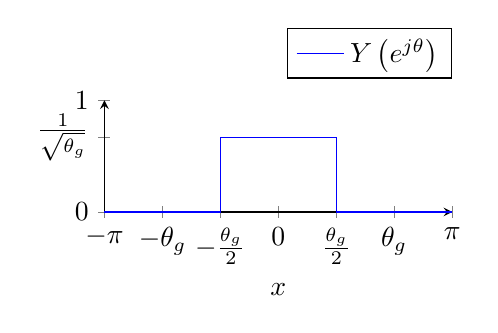
\begin{tikzpicture}
        \begin{axis}[
            domain=-pi:pi,
            axis x line=bottom, % no box around the plot, only x and y axis
            axis y line=left, % the * would suppress the arrow tips
            xlabel={$x$},
            ymax=1,
            legend style={at={(1,1.65), anchor=north west}},
            samples=50,
            height=3cm,
            width=6cm,
            xtick={-6.2831, -3.1416, -2.09, -1.05, 0, 1.05, 2.09, 3.1416, 6.2831},
            xticklabels={$-2\pi$,$-\pi$,$-\theta_g$,$-\frac{\theta_g}{2}$,$0$,$\frac{\theta_g}{2}$,$\theta_g$,$\pi$,$2\pi$},
            ytick={0,0.667,1},
            yticklabels={0,$\frac{1}{\sqrt{\theta_g}}$,1},
            clip=false]
            \addplot[mark=none, color=blue] coordinates {
                (-pi,0)
                (-pi/3,0)
                (-pi/3,2/3)
                (pi/3,2/3)
                (pi/3,0)
                (pi,0)
            };
            \addlegendentry[align=left]{$Y\left(e^{j\theta}\right)$};
        \end{axis}a
        \end{tikzpicture}}
        \raisebox{-.5\height}{$\xRightarrow{gefaltet}$}
        \raisebox{-.5\height}{
        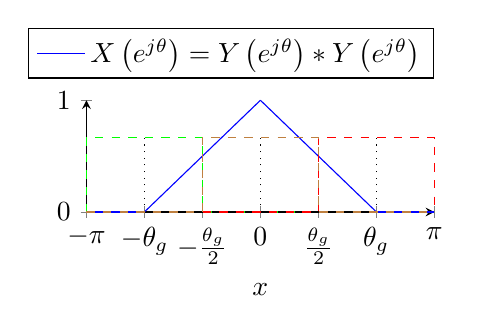
\begin{tikzpicture}
        \begin{axis}[
            domain=-pi:pi,
            axis x line=bottom, % no box around the plot, only x and y axis
            axis y line=left, % the * would suppress the arrow tips
            xlabel={$x$},
            ymax=1,
            legend style={at={(1,1.65), anchor=north west}},
            samples=50,
            height=3cm,
            width=6cm,
            xtick={-6.2831, -3.1416, -2.09, -1.05, 0, 1.05, 2.09, 3.1416, 6.2831},
            xticklabels={$-2\pi$,$-\pi$,$-\theta_g$,$-\frac{\theta_g}{2}$,$0$,$\frac{\theta_g}{2}$,$\theta_g$,$\pi$,$2\pi$},
            ytick={0,1},
            clip=false]
            \addplot[thin, smooth, blue,domain=0:2*pi/3] {1-3*x/(2*pi)};
            \addlegendentry[align=left]{$X\left(e^{j\theta}\right)=Y\left(e^{j\theta}\right)*Y\left(e^{j\theta}\right)$};
            \addplot[thin, smooth, blue,domain=-2*pi/3:0] {3*x/(2*pi)+1};
            \addplot[thin, smooth, blue,domain=2*pi/3:pi] {0};
            \addplot[thin, smooth, blue,domain=-pi:-2*pi/3] {0};

            \addplot[dotted, mark=none, color=black] coordinates {
                (0,0)
                (0,2/3)
            };
            \addplot[dotted, mark=none, color=black] coordinates {
                (-2*pi/3,0)
                (-2*pi/3,2/3)
            };
            \addplot[dotted, mark=none, color=black] coordinates {
                (2*pi/3,0)
                (2*pi/3,2/3)
            };

            \addplot[dashed,mark=none, color=green] coordinates {
                (-pi,0)
                (-pi,2/3)
                (-pi/3,2/3)
                (-pi/3,0)
                (pi,0)
            };
            \addplot[dashed,mark=none, color=red] coordinates {
                (-pi,0)
                (pi/3,0)
                (pi/3,2/3)
                (pi,2/3)
                (pi,0)
            };
            \addplot[dashed,mark=none, color=brown] coordinates {
                (-pi,0)
                (-pi/3,0)
                (-pi/3,2/3)
                (pi/3,2/3)
                (pi/3,0)
                (pi,0)
            };
        \end{axis}
        \end{tikzpicture}}

        Wenn 
        \[Y\left(e^{j\theta}\right)=\frac{1}{\sqrt{\theta_g}}
        \begin{cases}
            1& 0\leq|\theta|\leq\frac{\theta_g}{2}\\
            0& \frac{\theta_g}{2}<|\theta|<\pi\\
        \end{cases}\]
        dann ist die Faltung des Signals mit sich selbst ($\forall \theta_g<\pi$)
        \[X\left(e^{j\theta}\right)=Y\left(e^{j\theta}\right)*Y\left(e^{j\theta}\right)\]
        
        Nun haben wir das Signal und wir müssen es nur noch umtransformieren, um das Zeitsignal zu erhalten:
            \begin{definition}[Linearitätseigenschaft der Fouriertransformation]
                \[a_1x_1[n]+a_2x_2[n]\multimapdotbothA
                a_1X_1(e^{j\theta})+a_2X_2(e^{j\theta})\]
            \end{definition}

        \begin{uebsp_theory}
            Aus der Formelsammlung (Fouriertransformationspaare) folgt:
            \[\frac{\sin\alpha n}{\pi
                n},\;\;0<\alpha<\pi\;\;\;\multimapdotbothA\;\;\;X\left(e^{j\theta}\right)=
            \begin{cases}
                1& 0\leq|\theta|\leq\alpha\\
                0& \alpha<|\theta|<\pi\\
            \end{cases}\]
        \end{uebsp_theory}
        Somit können wir $Y\left(e^{j\theta}\right)\;\;\multimapdotbothB\;\;y[n]$ berechnen:
            \[Y\left(e^{j\theta}\right)=\frac{1}{\sqrt{\theta_g}}
        \begin{cases}
            1& 0\leq|\theta|\leq\frac{\theta_g}{2}\\
            0& \frac{\theta_g}{2}<|\theta|<\pi\\
    \end{cases}\;\;\;\multimapdotbothB\;\;\;\frac{1}{\sqrt{\theta_g}}\frac{\sin\frac{\theta_g}{2}}{\pi
n}=y[n]\]

        \begin{uebsp_theory}
                Aus der Formelsammlung (Fouriertransformation zeitdiskreter
                Signale) folgt:
                \[x[n]y[n]\;\;\;\multimapdotbothA\;\;\;\frac{1}{2\pi}\left(X\left(e^{j\theta}\right)*Y\left(e^{j\theta}\right)\right)\]
        \end{uebsp_theory}
        Somit können wir
        $X\left(e^{j\theta}\right)\;\;\;\multimapdotbothB\;\;\;x[n]$ berechnen:
        \[X\left(e^{j\theta}\right)=\frac{1}{2\pi}\left(Y\left(e^{j\theta}\right)*Y\left(e^{j\theta}\right)\right)\;\;\;\multimapdotbothB\;\;\;y[n]y[n]=\frac{x[n]}{2\pi}\]
        \[\;\;\Rightarrow\;\;
        2\pi\cdot
    X\left(e^{j\theta}\right)=\left(Y\left(e^{j\theta}\right)*Y\left(e^{j\theta}\right)\right)\;\;\;\multimapdotbothB\;\;\;2\pi\left(y[n]y[n]\right)=2\pi\left(y^2[n]\right)=x[n]\]
        \[\;\;\Rightarrow\;\;x[n]=2\pi\cdot
        \left(\frac{1}{\sqrt{\theta_g}}\frac{\sin\frac{\theta_g}{2}}{\pi
    n}\right)^2=\frac{2\cancel\pi\sin^2\frac{\theta_g}{2}}{\theta_g\cdot\pi^{\cancel{2}}n^2}
        =\frac{2\sin^2\frac{\theta_g}{2}}{\theta_g\cdot\pi n^2}\]

    \item ~\\
        \begin{center}
        \begin{tikzpicture}
        \begin{axis}[
            domain=-2*pi:2*pi,
            axis x line=bottom, % no box around the plot, only x and y axis
            axis y line=left, % the * would suppress the arrow tips
            xlabel={$x$},
            ymax=1,
            legend pos=north east,
            samples=50,
            height=3cm,
            width=12cm,
            xtick={-6.2831, -3.1416, 0, 3.1416, 6.2831},
            xticklabels={$-2\pi$,$-\pi$,$0$,$\pi$,$2\pi$},
            ytick={0,1},
            clip=false]
            \addplot[thin, smooth, blue,domain=0:pi] {1-x/(pi)};
            \addplot[thin, smooth, blue,domain=pi:2*pi] {2-x/(pi)};
            \addplot[thin, smooth, blue,domain=-pi:0] {-x/(pi)};
            \addplot[thin, smooth, blue,domain=-2*pi:-pi] {-1-x/(pi)};
            \addplot[mark=none, color=blue] coordinates {
                (-2*pi,1)
                (-2*pi,0)
            };
            \addplot[mark=none, color=blue] coordinates {
                (-pi,1)
                (-pi,0)
            };
            \addplot[mark=none, color=blue] coordinates {
                (0,1)
                (0,0)
            };
            \addplot[mark=none, color=blue] coordinates {
                (pi,1)
                (pi,0)
            };
            %\addlegendentry[align=left]{$\mathcal{N}(\muval, \sigmaval)$};
            %\draw [thick,dashed,black] (current axis.south-|{axis cs:\muval,0}) -- (current axis.north-|{axis cs:\muval,0}) node [above] {$\mu=\muval$};
        \end{axis}
        \end{tikzpicture}
        \end{center}

        Aufteilung von $X$ in $X_{pos}$ und $X_{neg}$:
        \[X\left(e^{j\theta}\right)=X_{pos}\left(e^{j\theta}\right)+X_{neg}\left(e^{j\theta}\right)\]
        \[X_{pos}=\frac{1}{2\pi}\int_{0}^{\pi}\left(1-\frac{\theta}{n}\right)e^{j\theta
        n} d\theta\]
        lt. Tutor soll das partiell integriert dann das folgende ergeben:

        \[\frac{1+jn\pi}{2\pi^2n^2}-\frac{(-1)^n}{2\pi^2n^2}\]

        Für die Berechnung von $X_{neg}$ reicht die Verschiebung im
        Frequenzbereich:
    \[X_{neg}[n]=X_{pos}(\theta+\pi)\;\;\Rightarrow\;\;x[n]=x_{pos}[n]+x_{neg}[n]=
        \begin{cases}x[n]=-\frac{1+(-1)^n}{j2\pi n}& \text{für } n\neq 0\\
        x[0]=\frac{1}{2} & \text{sonst}
    \end{cases}\]

    \attention{Bitte frage mich nie wie das genau gerechnet werden muss, denn ich
    weiß es nicht!!! (Aber scheinbar kommt sowas eh nicht zum Test)}
    \item $\displaystyle X\left(e^{j\theta}\right) =
        \frac{e^{-j\theta}}{1+\frac{1}{6}e^{-j\theta}-\frac{1}{6}e^{-j2\theta}}$

        Bei diesem Beispiel suchen wir ein Transformationspaar, das ähnlich, wie
        die Angabe aussieht:
        \begin{uebsp_theory}
            Aus der Formelsammlung (Fouriertransformationspaare) folgt:
            \[a^n\sigma[n],\;\;|a|<1\;\;\multimapdotbothA\;\;\frac{1}{1-ae^{-j\theta}}\]
        \end{uebsp_theory}
        Nun gilt es, unsere Formel so umzuformen, um dieses Transformationspaar
        verwenden zu können:

        \[X\left(e^{j\theta}\right) =
        \frac{e^{-j\theta}}{1+\frac{1}{6}e^{-j\theta}-\frac{1}{6}e^{-j2\theta}}\;\;\Rightarrow\;\;\fbox{Substituiere:
    $e^{-j\theta}=u$}\;\;\Rightarrow\;\;X\left(u\right) =
        \frac{u}{-\frac{1}{6}u^2+\frac{1}{6}u+1}\]

        \begin{definition}[Quadratische Lösungsformel]
            \[x_{1,2}=\frac{-b\pm\sqrt{b^2-4ac}}{2a}\]
        \end{definition}

        Bestimmen der Nullstellen, mittels der Quadratischen Lösungsformel:
        \begin{eqnarray*}
            u_{1,2}&=&\frac{-\frac{1}{6}\pm\sqrt{\left(\frac{1}{6}\right)^2+
                4\cdot\frac{1}{6}\cdot 1}}{-2\frac{1}{6}}
            =\frac{-\frac{1}{6}\pm\sqrt{\frac{1}{36}+
                \frac{4}{6}}}{-\frac{1}{3}}
            =\frac{-\frac{1}{6}\pm\sqrt{\frac{1}{36}+
                \frac{24}{36}}}{-\frac{1}{3}}
            =\frac{-\frac{1}{6}\pm\sqrt{\frac{25}{36}}}{-\frac{1}{3}}\\
            u_{1,2}&=&=\frac{-\frac{1}{6}\pm\frac{5}{6}}{-\frac{1}{3}}
            =\frac{\frac{1}{6}\mp\frac{5}{6}}{\frac{1}{3}}
            =3\left(\frac{1}{6}\mp\frac{5}{6}\right)
        \end{eqnarray*}
        \[u_1=3\frac{-4}{6}=\cancel3\frac{-2}{\cancel3}=-2\;\;\text{ und
        }\;\;u_2=3\frac{\cancel 6}{\cancel 6}=3\]

        Nun können wir uns die Faktoren ausdrücken, indem wir in $(u-u_1)$, bzw.
        $(u-u_2)$ einsetzen: 
        \[-\frac{1}{6}u^2+\frac{1}{6}u+1=(u+2)(u-3)x\]
        Berechnen des Korrekturfaktors $x$:
        \[-\frac{1}{6}u^2+\frac{1}{6}u+1=(u+2)(u-3)x\;\;\Rightarrow\;\;
            \frac{1}{6}\left(-u^2+u+6\right)=\left(u^2-3u+2u-6\right)x\]
            \[-\frac{1}{6}\cancel{\left(u^2-u-6\right)}=\cancel{\left(u^2-u-6\right)}x\;\;\Rightarrow\;\;x=-\frac{1}{6}\]

        \attention{Die Berechnung des Korrekturfaktors ist unbedingt notwendig,
            denn die Beziehung $a\cdot x^2+b\cdot x+c=(x-d)(x-e)$ gilt nur, wenn
        der Faktor $a=1$.}

        Jetzt können wir endlich die neue Form für $X(u)$ darstellen:
        \[X\left(u\right) =
        \frac{u}{-\frac{1}{6}u^2+\frac{1}{6}u+1}=\frac{u}{(u+2)(u-3)\left(-\frac{1}{6}\right)}=\frac{u}{(u+2)(u-3)}\left(-6\right)\]

        Nun müssen wir mittels Partialbruchzerlegung eine Summe erzeugen:
        \[\frac{u}{(u+2)(u-3)}\cancel{\left(-6\right)}=\left(\frac{A}{u+2}+\frac{B}{u-3}\right)\cancel{\left(-6\right)}\]
        \begin{eqnarray*}
            \frac{u}{(u+2)(u-3)}&=&\frac{A}{u+2}+\frac{B}{u-3}\\
            u&=&\frac{A\cancel{(u+2)}(u-3)}{\cancel{u+2}}+\frac{B(u+2)(\cancel{u-3})}{\cancel{u-3}}\\
            u&=&A(u-3)+B(u+2)
        \end{eqnarray*}
        Einsetzen der Nullstelle $u_1=-2$:
        \[u=A(u-3)+B(u+2)\;\;\Rightarrow\;\;-2=A(-2-3)+B(-2+2)\;\;\Rightarrow\;\;-2=A\cdot(-5)+B\cdot0\;\;\Rightarrow\;\;A=\frac{2}{5}\]
        Einsetzen der Nullstelle $u_2=3$:
        \[u=A(u-3)+B(u+2)\;\;\Rightarrow\;\;3=A(3-3)+B(3+2)\;\;\Rightarrow\;\;3=B\cdot
        5\;\;\Rightarrow\;\;B=\frac{3}{5}\]

        Einsetzen für $A$ und $B$ und dann besitzen wir endlich eine Äquivalente Summendarstellung unseres
        $X(u)$:
        \begin{eqnarray*}
            X\left(u\right) &=&
                \frac{u}{-\frac{1}{6}u^2+\frac{1}{6}u+1}=\frac{u}{(u+2)(u-3)}\left(-6\right)
            =\left(\frac{\frac{2}{5}}{u+2}+\frac{\frac{3}{5}}{u-3}\right)\left(-6\right)\\
            X\left(u\right) &=&
            \left(\frac{2}{u+2}+\frac{3}{u-3}\right)\left(-\frac{6}{5}\right)
            =\left(-\frac{6}{5}\right)\left(\frac{1}{\frac{u}{2}+1}+\frac{1}{\frac{u}{3}-1}\right)
    \end{eqnarray*}
        \begin{uebsp_theory}
            Aus der Formelsammlung (Fouriertransformationspaare) folgt:
            \[a^n\sigma[n],\;\;|a|<1\;\;\multimapdotbothA\;\;\frac{1}{1-ae^{-j\theta}}\]
        \end{uebsp_theory}
    Rücksubstituieren: $u=e^{-j\theta}$
        \begin{eqnarray*}
            X\left(e^{-j\theta}\right) &=&
            \left(-\frac{6}{5}\right)\left(\frac{1}{\frac{e^{-j\theta}}{2}+1}+\frac{1}{\frac{e^{-j\theta}}{3}-1}\right)=\frac{6}{5}\left(\frac{1}{\frac{-e^{-j\theta}}{2}-1}+\frac{1}{\frac{-e^{-j\theta}}{3}+1}\right)\\
            X\left(e^{-j\theta}\right) &=&
            \frac{6}{5}\left(\frac{1}{-1-\frac{1}{2}e^{-j\theta}}+\frac{1}{1-\frac{1}{3}e^{-j\theta}}\right)
            = 
            \frac{6}{5}\left(-\frac{1}{1+\frac{1}{2}e^{-j\theta}}+\frac{1}{1-\frac{1}{3}e^{-j\theta}}\right)\\
            X\left(e^{-j\theta}\right) &=&
            \frac{6}{5}\left(-\frac{1}{1-\left(-\frac{1}{2}\right)e^{-j\theta}}+\frac{1}{1-\frac{1}{3}e^{-j\theta}}\right)\;\;\multimapdotbothB\;\;
            \frac{6}{5}\left(-\left(-\frac{1}{2}\right)^n\sigma[n]+\left(\frac{1}{3}\right)^n\sigma[n]\right)
            = x[n]
    \end{eqnarray*}

    \[x[n]=\frac{6}{5}\left(\left(\frac{1}{3}\right)^n-\left(-\frac{1}{2}\right)^n\right)\sigma[n]\]
\end{enumerate}
\end{Answer}
\end{uebsp}


\end{document}
